\documentclass[tikz,border=8pt]{standalone}
% Shared look for every TikZ diagram. Load with \input{../../tools/tikz-style.tex}
\usepackage[sfdefault]{roboto}
\usetikzlibrary{arrows.meta, positioning, shapes.geometric, calc, fit, backgrounds}
\definecolor{cblue}{HTML}{4C78A8}
\definecolor{corange}{HTML}{F58518}
\definecolor{cgreen}{HTML}{54A24B}
\definecolor{cred}{HTML}{E45756}
\definecolor{cpurple}{HTML}{B279A2}
\definecolor{cgrey}{HTML}{6B6B6B}
\tikzset{
  every picture/.style={font=\sffamily, line width=1.2pt},
  box/.style={draw=#1, fill=#1!12, rounded corners=4pt, align=center, inner sep=7pt, minimum height=1.1cm},
  box/.default=cgrey,
  arrow/.style={-{Stealth[length=3mm]}, draw=cgrey, line width=1.4pt},
  title/.style={font=\sffamily\bfseries\Large},
  note/.style={font=\sffamily\small, text=cgrey, align=center},
}
\AtBeginDocument{\hyphenpenalty=10000 \exhyphenpenalty=10000}

% A laser beam passes through glass and reports the maximum range, as the glass pane of the range-sensor Note (RO-010)
% shows; an ultrasonic pulse echoes off glass (Barreto-Cubero et al. 2021). The ultrasonic cone is 20 to 40 degrees
% wide (Correll 5.4); 30 degrees is drawn.
\begin{document}
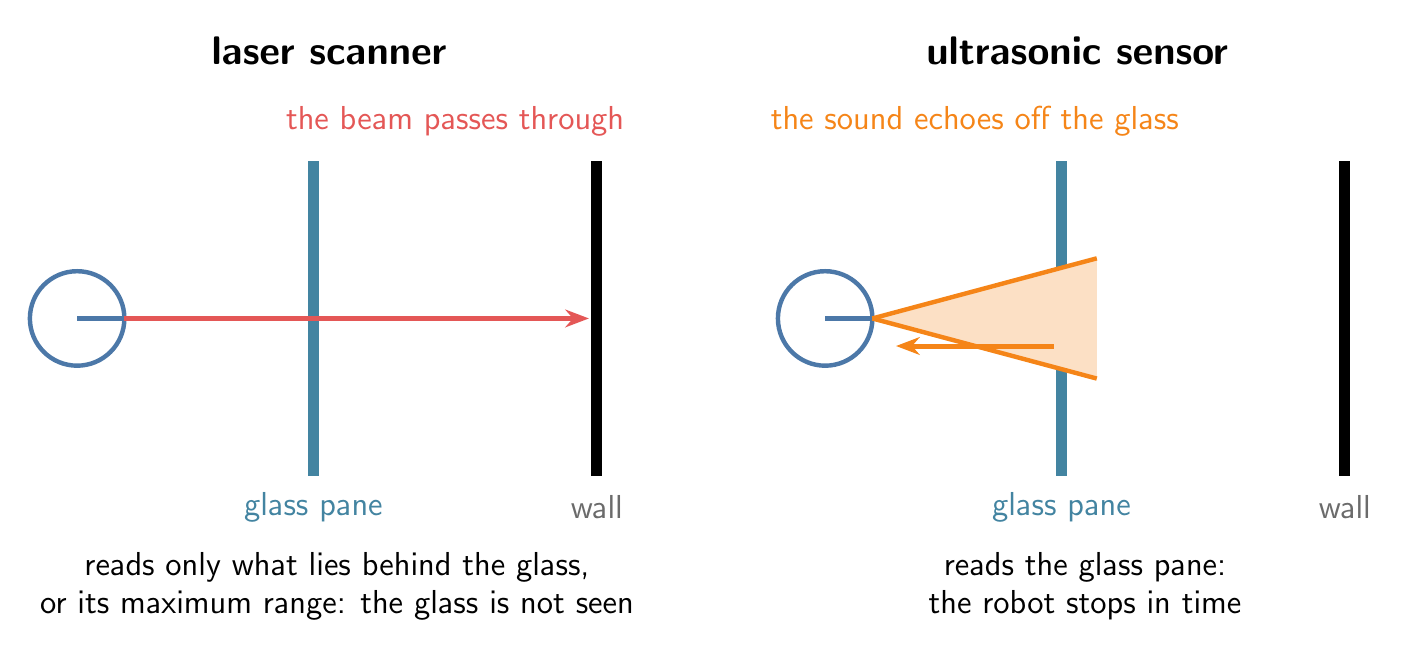
\begin{tikzpicture}
  \foreach \x/\ttl in {0/laser scanner, 9.5/ultrasonic sensor} {
    \begin{scope}[shift={(\x,0)}]
      \node[title] at (3.2,3.4) {\ttl};
      \draw[cblue, line width=1.6pt, fill=white] (0,0) circle (0.6);
      \draw[cblue, line width=2pt] (0,0) -- (0.6,0);
      \draw[cyan!60!black, line width=4pt] (3.0,-2.0) -- (3.0,2.0);
      \node[note, font=\sffamily\large, text=cyan!60!black] at (3.0,-2.4) {glass pane};
      \draw[black, line width=4pt] (6.6,-2.0) -- (6.6,2.0);
      \node[note, font=\sffamily\large] at (6.6,-2.4) {wall};
    \end{scope}}
  % laser
  \draw[cred, line width=1.8pt, -{Stealth[length=3mm]}] (0.6,0) -- (6.5,0);
  \node[note, font=\sffamily\large, text=cred, align=center] at (4.8,2.5) {the beam passes through};
  \node[note, font=\sffamily\large, text=black, align=center] at (3.3,-3.4) {reads only what lies behind the glass,\\ or its maximum range: the glass is not seen};
  % ultrasonic
  \fill[corange!25] (10.1,0) -- ($(10.1,0)+(15:2.95)$) -- ($(10.1,0)+(-15:2.95)$) -- cycle;
  \draw[corange, line width=1.6pt] (10.1,0) -- ($(10.1,0)+(15:2.95)$); \draw[corange, line width=1.6pt] (10.1,0) -- ($(10.1,0)+(-15:2.95)$);
  \draw[corange, line width=1.8pt, -{Stealth[length=3mm]}] (12.4,-0.35) -- (10.4,-0.35);
  \node[note, font=\sffamily\large, text=corange, align=center] at (11.4,2.5) {the sound echoes off the glass};
  \node[note, font=\sffamily\large, text=black, align=center] at (12.8,-3.4) {reads the glass pane:\\ the robot stops in time};
\end{tikzpicture}
\end{document}
